\documentclass[12pt, a4paper, oneside]{ctexart}
\usepackage{amsmath, amsthm, amssymb, bm, color, framed, graphicx, hyperref, mathrsfs}

\title{\textbf{随机过程作业14}}
\author{周强(119) \ 电子学院 \ \ \  202128019427002}
\date{\today}
\linespread{1.5}
\definecolor{shadecolor}{RGB}{241, 241, 255}
\newcounter{problemname}
\newenvironment{problem}{\begin{shaded}\stepcounter{problemname}\par\noindent\textbf{题目\arabic{problemname}. }}{\end{shaded}\par}
\newenvironment{solution}{\par\noindent\textbf{解答. }}{\par}
\newenvironment{note}{\par\noindent\textbf{题目\arabic{problemname}的注记. }}{\par}

\begin{document}

\maketitle

\begin{problem}
    设 $X_{n}=\sum_{k=1}^{N} \sigma_{k} \sqrt{2} \cos \left(\alpha_{k} n-U_{k}\right)$, 其中 $\sigma_{k}$ 和 $\alpha_{k}$ 为正常数, $U_{k} \sim U(0,2 \pi)$, 且相互 独立, $k=1,2, \cdots, N$, 试计算 $\left\{X_{n}, n=0, \pm 1, \cdots\right\}$ 的均值函数和相关函数, 并说明其是 否是平稳过程。
\end{problem}

\begin{solution}
    $X_n$的均值函数为
    \begin{align*}
        & E\{
            X_n
        \}
        =
        E\left\{
            \sum_{k=1}^{N} \sigma_{k} \sqrt{2} \cos \left(\alpha_{k} n-U_{k}\right) 
        \right\}
        \\
        & =
        \sum_{k=1}^{N} \sigma_{k}\sqrt{2}
        E\left\{
              \cos \left(\alpha_{k} n-U_{k}\right) 
        \right\}
        = 0
    \end{align*}
    $X_n$的相关函数为
    \begin{align*}
        R_X(n,m) 
        & = 
        E\left\{
            X_n \cdot X_m
        \right\}
        \\
        & =
        E\left\{
            \left[
            \sum_{k=1}^{N} \sigma_{k} \sqrt{2} \cos \left(\alpha_{k} n-U_{k}\right)
            \right] 
            \cdot
            \left[
            \sum_{j=1}^{N} \sigma_{j} \sqrt{2} \cos \left(\alpha_{j} m-U_{j}\right)
            \right] 
        \right\}
        \\
        & =
        E \left\{
            2
            \sum_{k=1}^{N}{
                \sum_{j=1}^{N}{
                    \sigma_{k} \sigma_{j}
                    \cos \left(\alpha_{k} n-U_{k}\right)
                    \cos \left(\alpha_{j} m-U_{j}\right)
                }
            }
        \right\}
        \\
        & =
        E \left\{
            2
                \sum_{j=1}^{N}{
                    \sigma_{j}^2
                    \cos \left(\alpha_{j} n-U_{j}\right)
                    \cos \left(\alpha_{j} m-U_{j}\right)
                }
        \right\}
        \\
        & =
            2
            \sum_{j=1}^{N}{
                \sigma_{j}^2
                E \left\{
                \cos \left(\alpha_{j} n-U_{j}\right)
                \cos \left(\alpha_{j} m-U_{j}\right)
                \right\}
            }
            \\
            & =
                \sum_{j=1}^{N}{
                    \sigma_{j}^2
                    E \left\{
                    \cos \left(\alpha_{j} (n+m)-2U_{j}\right)
                    +
                    \cos \left(\alpha_{j} (n-m)\right)
                    \right\}
                }
            \\
            & =
            \sum_{j=1}^{N}{
                \sigma_{j}^2
                \cos \left(\alpha_{j} (n-m)\right)
            }
    \end{align*}
    由上述计算可知,$X_n$的均值函数与时间无关,相关函数仅与时间差有关。因此$X_n$是平稳过程。
\end{solution}

\begin{problem}
    设有随机过程 $X(t)=A \cos (\omega t+\pi \eta(t))$, 其中 $\omega>0$ 为常数, $\{\eta(t), t \geq 0\}$ 是泊松过程, $A$ 是与 $\eta(t)$ 独立的随机变量, 且 $P\{A=-1\}=P\{A=1\}=1 / 2$ 。
    \begin{itemize}
        \item[(1)] 试画出此过程的样本函数, 并问样本函数是否连续?
        \item[(2)] 试求此过程的相关函数, 并问该过程是否均方连续?
    \end{itemize}
\end{problem}

\begin{solution}
某个典型的样本函数如下图所示,其中实线部分代表样本函数,虚线部分是样本函数关于X轴对称的图像,仅仅是为了观察方便。由下图可知,样本函数不连续。
\\
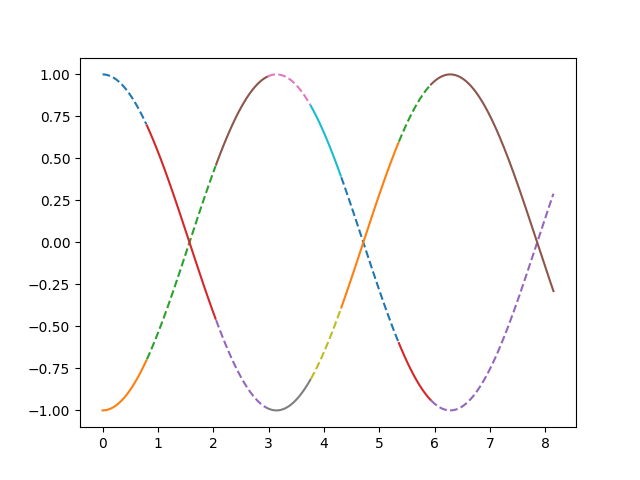
\includegraphics[scale=0.8]{Figure_1.png}

$X(t)$ 的相关函数如下

\begin{align*}
    R_X(t_1, t_2)
    & =
    E\{
        A \cos (\omega t_1 + \pi \eta(t_1))  
        \cdot
        A \cos (\omega t_2 + \pi \eta(t_2)) 
    \}
    \text{(独立性)}
    \\
    & =
    E\{A^2\}
    E\{
        \cos (\omega t_1 + \pi \eta(t_1))  
        \cdot
        \cos (\omega t_2 + \pi \eta(t_2)) 
    \}
    (\text{积化和差,}E\{A^2\}=1)
    \\
    & =
    \frac{1}{2}
    E\{
        \cos (\omega (t_1+t_2) + \pi [\eta(t_1) + \eta(t_2)])  
        +
        \cos (\omega (t_1-t_2) + \pi [\eta(t_1) - \eta(t_2)]) 
    \}
    \\
    & =
    \frac{1}{2}
    E\{
        \cos (\omega (t_1+t_2) + \pi [\eta(t_1) - \eta(t_2)])  
        +
        \cos (\omega (t_1-t_2) + \pi [\eta(t_1) - \eta(t_2)]) 
    \}
    \text{期望定义}
    \\
    & =
    \frac{1}{2}
    \sum_{k=0}^{\infty}{
        (-1)^k
        [
        \cos(\omega (t_1+t_2))
        +
        \cos(\omega (t_1-t_2))
        ]
        \frac{(\lambda (t_1-t_2))^{k}}
        {k!}
        e^{
            -\lambda (t_1-t_2)
        }
    }
    \text{泰勒展开}
    \\
    & =
    \frac{1}{2}
    [
        \cos(\omega (t_1+t_2))
        +
        \cos(\omega (t_1-t_2))
    ]
    e^{
        -2\lambda (t_1-t_2)
    }
    \\
    & =
    \cos \omega t_{1} \cos \omega t_{2} \cdot e^{-2 \lambda\left(t_{2}-t_{1}\right)}
\end{align*}
\\
该过程是均方连续的随机过程
\end{solution}
\end{document}